\documentclass[fontsize=11pt,a4paper,final]{scrartcl}[2003/01/01]
\usepackage[ngerman]{babel} 
\usepackage[utf8]{inputenc} 
\usepackage[autostyle=true,german=quotes]{csquotes}
\usepackage[T1]{fontenc}
\usepackage{float}
\usepackage{floatflt}
\usepackage{listings}
\usepackage[hidelinks]{hyperref}
\usepackage{tabularx}
\usepackage[sort&compress,numbers]{natbib}
\usepackage{caption}
\usepackage{listings}
\usepackage{color}

\captionsetup[table]{skip=0pt}
\captionsetup[figure]{skip=10pt}

\title{Embedded Systems Dokumentation}
\author{Von Christian Weber und Manuel Wurth}
\date{\today}

%Bilder scalen, wenn größer als Seite
\usepackage[final]{graphicx}
\makeatletter
\def\ScaleIfNeeded{%
	\ifdim\Gin@nat@width>\linewidth
		\linewidth
	\else
		\Gin@nat@width
	\fi
}
\makeatother

\newcommand*{\quelle}{% 
	\footnotesize Quelle: 
}

\newcommand*{\manu}{%
	Programmiert von: Manuel Wurth
}

\newcommand*{\chris}{%
	Programmiert von: Christian Weber
}

\definecolor{mygreen}{rgb}{0,0.6,0}
\definecolor{mygray}{rgb}{0.5,0.5,0.5}
\definecolor{mymauve}{rgb}{0.58,0,0.82}

\lstset{
  backgroundcolor=\color{white},   % choose the background color; you must add \usepackage{color} or \usepackage{xcolor}
  basicstyle=\footnotesize,        % the size of the fonts that are used for the code
  breakatwhitespace=false,         % sets if automatic breaks should only happen at whitespace
  breaklines=true,                 % sets automatic line breaking
  captionpos=b,                    % sets the caption-position to bottom
  commentstyle=\color{mygreen},    % comment style
  escapeinside={\%*}{*)},          % if you want to add LaTeX within your code
  extendedchars=true,              % lets you use non-ASCII characters; for 8-bits encodings only, does not work with UTF-8
  frame=single,	                   % adds a frame around the code
  keepspaces=true,                 % keeps spaces in text, useful for keeping indentation of code (possibly needs columns=flexible)
  keywordstyle=\color{blue},       % keyword style
  language=C,                 	   % the language of the code
  otherkeywords={*,...},           % if you want to add more keywords to the set
  numbers=left,                    % where to put the line-numbers; possible values are (none, left, right)
  numbersep=5pt,                   % how far the line-numbers are from the code
  rulecolor=\color{black},         % if not set, the frame-color may be changed on line-breaks within not-black text (e.g. comments (green here))
  showspaces=false,                % show spaces everywhere adding particular underscores; it overrides 'showstringspaces'
  showstringspaces=false,          % underline spaces within strings only
  showtabs=false,                  % show tabs within strings adding particular underscores
  stepnumber=1,                    % the step between two line-numbers. If it's 1, each line will be numbered
  stringstyle=\color{mymauve},     % string literal style
  tabsize=2,	                   % sets default tabsize to 2 spaces
  caption=\lstname                 % show the filename of files included with \lstinputlisting; also try caption instead of title
}

\begin{document}
	
\maketitle
\newpage
\tableofcontents
\newpage

\section{Simulator}
Weil die Gruppenzahl zu hoch ist, als dass ausreichend oft auf die Hardware zugegriffen werden könnte, haben wir uns entschlossen die Anlage zu simulieren. Als erstes wurde ein C-Simulator geschrieben, allerdings hat sich nach einiger Zeit herausgestellt, dass dieser für eine genauere Analyse von Fehlern unvorteilhaft ist. 
Deshalb wurde die Entwicklung nach einiger Zeit eingestellt und ein Java-Simulator mit grafischer Oberfläche entwickelt.

\subsection{C-Simulator (verworfen) - \manu}

\begin{figure}[H]
	\centering
	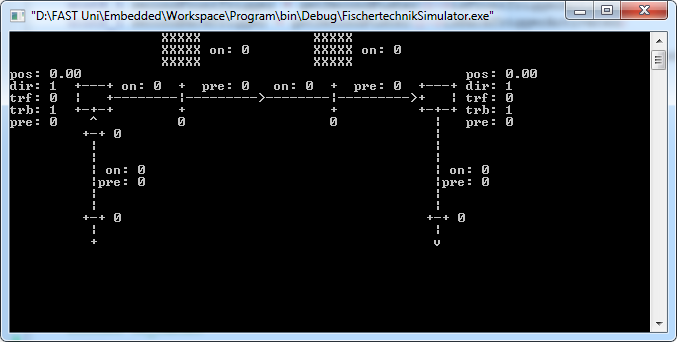
\includegraphics[width=1\ScaleIfNeeded]{Bilder/C-Simulator.png}
	\caption{Der C-Simulator}
	\label{fig:C-Simulator}
\end{figure} \ \\
\noindent Die Ausgabe des Simulators ist in Abbildung \ref{fig:C-Simulator} dargestellt. Ziel war es, die Anlage mit allen relevanten Informationen mithilfe von ASCII-Zeichen darzustellen. Darunter alle Lichtschranken, \textit{flags}, die anzeigen ob eine Station gerade belegt ist (pre), die beiden Schieber mit ihren Daten und die beiden Werkzeuge. \\ \\
Der Simulator war ursprünglich nur für Situationen geplant, an denen jede Station höchstens ein Werkstück bearbeitet. Dafür war die Darstellung noch ausreichend und die Logik konnte getestet werden. Für mehr als ein Werkstück pro Station wird die Darstellung aber schnell sehr unübersichtlich, deshalb haben wir uns dazu entschieden an einer grafischen Lösung zu arbeiten. Dieser Simulator wird also nicht mehr verwendet, deshalb wird hier auf Codebeispiele verzichtet, auch um Platz für andere Teilbereiche zu sparen, die tatsächlich zum Einsatz kommen.
\subsection{Java-Simulator}
\chris

\section{Architektur}
\chris
\section{Modi (States)}
TODO: Bild von Automaten?
\subsection{Not Aus}
\chris
\subsection{Diagnose}
\chris

\subsection{Inbetriebnahme}
\subsection{Normalbetrieb (\manu)}
Dieses Kapitel widmet sich der Umsetzung des Normalbetriebs der Anlage. Um den Umfang der Dokumentation klein zu halten, werden nur interessante Aspekte beleuchtet.
\begin{lstlisting}[caption={Beispiel: Struct für die erste \textit{stage} (erstes Laufband)},label={lst:strukt1}]
typedef struct
{
	short itemCount;
	int itemPositions[3];
	short firstLightBarrierBefore;
	short secondLightBarrierBefore;
	short isRunning;
	short timeout;
	short hasItemPassedSecondLB;
} StageOne;
\end{lstlisting} 
Die Anlage wurde in 6 \textit{stages} unterteilt, die jeweils eigenständig und mit Rücksicht auf die nächste \textit{stage} arbeiten. Für jede \textit{stage} wurden \lstinline|structs| angelegt, die alle Daten halten, die für den Betrieb der \textit{stage} erforderlich sind (siehe z.B. in Listing \ref{lst:strukt1}). Eigenständige \textit{stages} sind die vier Laufbänder sowie die beiden Schieber, jeweils inklusive aller Sensoren und Aktoren. Der Normalbetrieb erfolgt unter Berücksichtigung einer ganz bestimmten Reihenfolge von Aktionen:
\begin{enumerate}
\item Sensoren lesen
\item Berechnungen jeder \textit{stage} für die Aktoren
\item Aktoren steuern
\end{enumerate}

\subsubsection{Werkstücke und Positionen}
Damit zu jeder Zeit Staus erkannt und Kollisionen/Berührungen von Werkstücken verhindert werden können, musste eine geeignete Lösung gefunden werden. Damit die Funktionalität der Lichtschranken gewährleistet werden kann, also ein \textit{toggeln} noch stattfindet, muss ein ausreichend großer Abstand zwischen den Werkstücken eingehalten werden. Bei 3 Werkstücken pro Laufband kann dies gerade noch erreicht werden, vorausgesetzt die Abstände sind gleich groß. Die Abstände zwischen den Werkstücken sind ab dem ersten Schieber von den \textit{ready}-Zuständen der einzelnen \textit{stages} abhängig, die im Folgenden beschrieben werden. Ist eine \textit{stage ready}, kann die Vorgänger-\textit{stage} ein Werkstück weitertransportieren und übergeben. \\ \\
\textbf{Wann ist Laufband 1 ready?} \\
Die Bestimmung des \textit{ready-flags} des ersten Laufbands ist am trivialsten, weil es schlicht nicht existiert. Das \textit{flag} soll der Vorganger-\textit{stage} signalisieren, dass die \textit{stage} bereit für ein neues Werkstück ist. Laufband 1 hat keine Vorgänger-\textit{stage}; alleine der Bediener der Anlage bestimmt, wann ein neues Werkstück aufgelegt wird. \\ \\
\textbf{Wann sind die beiden Schieber \textit{ready}?}
\begin{lstlisting}[caption={Beispiel: \textit{ready-flag} des ersten Schiebers},label={lst:schieber-ready}]
if(stageTwo.isOccupied || getFirstPusher()->isBackTriggerActivated != 1)
{
   	stageTwo.isReady = 0;
}
else
{
   	stageTwo.isReady = 1;
}
\end{lstlisting} 
Ein Schieber ist immer dann für ein neues Werkstück bereit, wenn er nicht belegt und vollständig zurück gefahren ist (siehe Listing \ref{lst:schieber-ready}). \\ \\
\textbf{Wann sind die Laufbänder 2 und 3 \textit{ready}?} \\ \\
Für die ersten drei Laufbänder werden die (ungefähren) Positionen der auf ihnen beförderten Werkstücke gespeichert. Damit dies ausreichend genau festgelegt werden kann, wird die Position nicht schon bei der Übergabe auf das Laufband gesetzt. Hier kann es nämlich passieren, dass das Werkstück nicht sofort vom Laufband aufgenommen wird. Diese Varianz der tatsächlichen Positionen kann für die Ausführung gefährlich werden, deshalb wurde eine andere Herangehensweise erdacht.
\begin{lstlisting}[caption={Beispiel: Neues Werkstück auf dem zweiten Laufband},label={lst:neuesItem2}]
// check if new item
if(stageThree.itemCount > stageThree.itemCountBefore)
{
   	// new item
   	stageThree.itemCountBefore = stageThree.itemCount;
   	
   	short i = 0;
   	for( i ; i < 3 ; i++)
   	{
   		if(stageThree.itemPositions[i] == -1)
   		{
   			stageThree.itemPositions[i] = -2;
   			break;
   		}
   	}
}
\end{lstlisting}
Als Beispiel eines neuen Werkstücks auf dem zweiten Laufband, kann Listing \ref{lst:neuesItem2} herangezogen werden.
Soll ein Werkstück an die nächste \textit{stage} übergeben werden, wird einfach deren \lstinline|itemCount| inkrementiert. Die nachfolgende \textit{stage} merkt dies, weil sie stets ihren alten \lstinline|itemCount| kennt (Zeile 2). \\
Als nächstes wird ein freier Slot für das neue Werkstück gesucht. Freie Slots haben immer den Wert $-1$ (Zeilen 8 - 10). An dieser Stelle könnte man nun die neue Position des Werkstücks auf $0$ setzten, weil es sich schließlich am Anfang des Laufbands befinden muss. Alle Positionen die größer als $-1$ sind werden automatisch inkrementiert, wenn sich das Laufband bewegt. In diesem Fall wäre das aus den oben genannten Gründen aber problematisch. Deshalb bekommt das neue Werkstück die Platzhalter-Position $-2$ (Zeile 12). Diese bedeutet, dass sich ein Werkstück auf dem Laufband, genauer, vor der zentralen Lichtschranke befindet. 
Sobald das Werkstück die Mitte der Lichtschranke (wo sich der Bohrer befindet) erreicht, kann die Position des Werkstücks sehr genau bestimmt und gesetzt werden. \\ \\
Doch was hat das mit dem \textit{ready-flag} zu tun? 
\begin{lstlisting}[caption={Beispiel: Ist Laufband 2 \textit{ready}?},label={lst:ready2}]
stageThree.isReady = 1;
short i = 0;
for(i ; i < 3 ; i++)
{
	if(stageThree.itemPositions[i] == -2)
	{
		stageThree.isReady = 0;
		break;
	}
}
\end{lstlisting}
Die \textit{stage} ist immer genau dann \textit{ready}, wenn sich kein Werkstück auf dem Laufband vor der Lichtschranke befindet (siehe Listing \ref{lst:ready2}). \\ \\
\textbf{Wann ist Laufband 4 \textit{ready}?} \\
Das letzte Laufband ist immer dann \textit{ready}, wenn die anliegende Lichtschranke nicht länger als ein einstellbarer Wert blockiert ist. Ist das Laufband leer, kann ein Werkstück die Lichtschranke passieren, ohne dass sich das \textit{ready-flag} ändert. Befindet sich bereits ein Werkstück hinter der Lichtschranke, würde ein weiteres Werkstück die Lichtschranke länger blockieren und das \textit{ready-flag} toggeln. \\ 
Ab diesen Zeitpunkt fährt das Laufband in regelmäßigen Abständen kurz an, um zu prüfen, ob ein Werkstück herausgenommen wurde. Ist dies der Fall wird die Lichtschranke wieder frei und die \textit{stage} ist erneut \textit{ready}. \\ \\
\textbf{Wo soll ein Werkstück auf eine nächste \textit{stage} warten?} \\
Für das erste Laufband hat sich die zweite Lichtschranke als eine gute Warteposition herausgestellt. Die Laufbänder 2 und 3 lassen ihre Werkstücke bei $70\%$ der Laufbandlänge warten. Der zweite Schieber kann so gerade noch ohne Kontakt zum wartenden Werkstück bewegt werden, was der maximalen Nutzung des Laufbands entgegenkommt.

\subsubsection{Störfälle erkennen}
Die Anlage soll erkennen, wenn Werkstücke verloren gehen oder Lichtschranken unerwartet auslösen. 
\\ \\
\textbf{Werkstück geht verloren}
\begin{lstlisting}[caption={Beispiel: Werkstück geht auf ersten Laufband verloren},label={lst:itemLost}]
if(stageOne.isRunning)
{
   	stageOne.timeout += totalSystem.timeDiffSinceLastCall;
}
if(stageOne.timeout >= TIMEOUT)
{
   	timeout(1);
}
if(getSecondLightBarrier()->isBlocked || stageOne.itemCount == 0)
{
   	stageOne.timeout = 0;
}
\end{lstlisting}
Solange die \textit{stage} denkt, es liegt ein Werkstück auf ihr, wird sie versuchen es zu transportieren. Listing \ref{lst:itemLost} zeigt was passiert, wenn ein Werkstück auf dem ersten Laufband auf dem Weg von der ersten zur zweiten Lichtschranke verloren geht. Immer wenn sich das Laufband bewegt, wird ihr eigener \textit{timeout}-Wert um die vergangene Zeit seit dem letzten Aufruf erhöht (Zeilen 1 - 4). Sobald die zweite Lichtschranke blockiert wird oder sich keine Werkstücke auf dem Laufband befinden, wird dieser Wert wieder auf $0$ zurückgesetzt (Zeilen 9 - 12). Erreicht der Wert allerdings eine einstellbare Schwelle, wird die Funktion \lstinline|timeout()| aufgerufen, die einen Notaus in die Wege leitet (Zeilen 5 - 8). Auf ähnliche Weise wird für alle \textit{stages} mit Laufband vorgegangen. Schieber besitzen keine Sensoren zur Werkstückerkennung.\\ \\
\textbf{Lichtschranke wird unerwarteterweise ausgelöst}

\begin{lstlisting}[caption={Beispiel: Zweite Lichtschranke wird unerwartet ausgelöst},label={lst:unexpectedItem}]
if((stageOne.itemCount == 0 || stageOne.itemCount == 1 && stageOne.hasItemPassedSecondLB) && getSecondLightBarrier()->isBlocked)
{
	unexpectedItem(2);
}
\end{lstlisting}
Als Beispiel für eine unerwartet ausgelöste Lichtschranke soll Listing \ref{lst:unexpectedItem} herangezogen werden. Wird die zweite Lichtschranke des ersten Laufbands \underline{unerwartet} ausgelöst, liegt entweder kein Werkstück auf dem Laufband oder es liegt genau ein Werkstück auf dem Laufband, und zwar hinter der zweiten Lichtschranke (Zeile 1). Ist dies der Fall, wir die Funktion \lstinline|unexpectedItem()| ausgeführt, die abermals zu einem Notaus führt.

\subsection{Pause und Stopp}
Um Gegensatz zu den anderen Modi muss bei den Modi Pause und Stopp der aktuelle Zustand des laufenden Betriebs erhalten bleiben. Es hat sich deshalb angeboten, beide Modi als Teil des laufenden Betriebs zu etablieren.

\begin{lstlisting}[caption={Die Funktion \lstinline|runningComputeActions|},label={lst:runningComputeActions}]
void runningComputeActions() {
	computeFirstTreadmill();
	computeFirstPlate();
	computeSecondTreadmill();
	computeThirdTreadmill();
	computeSecondPlate();
	computeFourthTredmill();
	computeRestState();
	computeStopState();
	computeErrorCases();
}
\end{lstlisting}
Um zu verstehen, in welcher Reihenfolge die Berechnungen für die Aktoren stattfinden, muss die Funktion \lstinline|runningComputeActions()| begutachtet werden (Siehe Listing \ref{lst:runningComputeActions}). Die Berechnungen der einzelnen \textit{stages} ist voneinander unabhängig. Eine bestimmte Reihenfolge ist nicht wichtig, weil sie nur ihren eigenen Status manipulieren (Ausnahme: \lstinline|itemCount| der nächsten \textit{stage}). Die beiden Modi Pause und Stopp regeln aber potentiell alle Aktoren, also müssen sie die Berechnungen der \textit{stages} überschreiben können. Deshalb kommt deren Berechnung erst nach den Berechnungen der \textit{stages} (Zeilen 8 und 9). \\ \\
\textbf{Modus Pause}
\begin{lstlisting}[caption={Die Pause Funktion},label={lst:rest}]
void computeRestState()
{
	if(getSiteState() == REST)
	{
		stageOne.isRunning = 0;
		stageThree.isTMRunning = 0;
		stageFour.isTMRunning = 0;
		stageSix.isRunning = 0;
	}
}
\end{lstlisting}
Alle Laufbänder werden angehalten, Schieber, Bohrer und Fräse beenden angefangene Arbeitsschritte (siehe Listing \ref{lst:rest}). \\ \\
\textbf{Modus Stopp}
\begin{lstlisting}[caption={Die Stopp Funktion},label={lst:stop}]
void computeStopState()
{
	if(getSiteState() == STOP && getFirstLightBarrier()->isBlocked && stageOne.itemCount == 1)
	{
		stageOne.isRunning = 0;
	}
}
\end{lstlisting}
Die Anlage wird kontrolliert und ohne Ausschluss leer gefahren. Sobald das erste Laufband frei ist werden keine weiteren Werkstücke mehr angenommen (siehe Listing \ref{lst:stop}).
\section{Kommunikation}

\end{document}